\chapter{Results} \label{sec:6} This chapter presents the results obtained from
the case study discussed in the previous chapter.

\section{EvoDrawing01}

Experiment ED01 generated a user-model graph with the following data
presented(Table\ref{tab:dataGenerated_1}).

\begin{table}
\small
\caption{Data generated in the graph-based user model.}
\label{tab:dataGenerated_1}
\centering
\small
\begin{tabular}{p{3cm} p{3cm} p{3cm} }
\hline\noalign{\smallskip}
  & Data &  \\
\noalign{\smallskip}\hline\noalign{\smallskip}
\small{Nodes} & \small{595} & \\ \hline
\small{Relationships} & \small{2220} & \\ \hline

\noalign{\smallskip}\hline
\end{tabular}
\end{table}


This data is the total of nodes as well as their relationships. Also in
Table~\ref{tab:totalUsers_12} is shown the total of volunteer active users.

\begin{table}
\small
\caption{Total number of volunteers active users.}
\label{tab:totalUsers_12}
\centering
\small
\begin{tabular}{p{3cm} p{3cm} p{3cm} }
\hline\noalign{\smallskip}
  & Users &  \\
\noalign{\smallskip}\hline\noalign{\smallskip}
\small{Total } & \small{53} & \\ \hline
\noalign{\smallskip}\hline
\end{tabular}
\end{table}

In order to observe which users have better social interconnectivity within the
experiments it was decided to make a relation of number known users that the
user’s have. This relation is shown in table \ref{tab:knownUsers_1}

\begin{table}
\small
\caption{Number of known among users.}
\label{tab:knownUsers_1}
\centering
\small
\begin{tabular}{p{3cm} p{3cm}  }
\hline\noalign{\smallskip}
 User name & Number of known users \\
\noalign{\smallskip}\hline\noalign{\smallskip}
\small{Chriss de Blanc } & \small{7}  \\ \hline
\small{Alejandro Salcido } & \small{4}  \\ \hline
\small{Jonathan Amezcua Aguiluz } & \small{1}  \\ \hline
\small{Daniela Sanchez } & \small{1}  \\ \hline
\small{Jennifer Llamas} & \small{1}  \\ \hline
\small{Iliana Dl } & \small{1}  \\ \hline
\small{Xochilt Ramirez Garcia } & \small{1}  \\ \hline
\small{Manuel Elizondo } & \small{1}  \\ \hline
\small{Julian Torres } & \small{1}  \\ \hline
\small{Data Back } & \small{1}  \\ \hline
\small{Frank Arce } & \small{1}  \\ \hline
\small{Gustavo Vargas } & \small{1}  \\ \hline
\noalign{\smallskip}\hline
\end{tabular}
\end{table}

Likewise in Table~\ref{tab:knownUsers_1} the interconnectivity that particular
user has with other users is shown. The degree of relationship of users is
associated with the number of friends known within the application. This means
that a degree of influence is among participants. For example  "Chriss
Blanc" user has a degree of relatedness 7 as shown in Figure
\ref{fig:guserknown_1} indicating that this particular user can have more
influence on the decisions of others. Moreover the user ``Alejandro Salcido'' has
the second highest degree of relationship to other users as shown in Figure
\ref{fig:guserknown_1}.

\begin{figure*}
%\captionsetup{justification=centering,margin=1cm}
\centering
\fbox{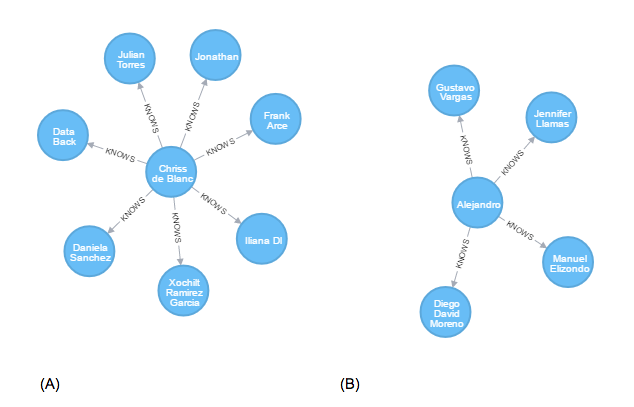
\includegraphics[scale=0.75]{img/users_known_1.PNG}} %[width=0.7\textwidth]
\caption{Graph users with greater interconnectivity.}
\label{fig:guserknown_1}
\end{figure*}

Figure\ref{fig:guserknown_1} shows those users more connected in the graph. This
may represent the degree of impact of a user and the possible influence that may
have on the decisions of other users. For example, if the user with the greatest
impact is affected in any decision likely other users may be affected in some
way.


\begin{table}
\small
\caption{Total number of individuals generated.}
\label{tab:totalIndividuals_12}
\centering
\small
\begin{tabular}{p{3cm} p{3cm} p{3cm} }
\hline\noalign{\smallskip}
  & Individuals &  \\
\noalign{\smallskip}\hline\noalign{\smallskip}
\small{Total } & \small{500} & \\ \hline
\noalign{\smallskip}\hline
\end{tabular}
\end{table}


Table \ref{tab:totalIndividuals_12} presents the total number of individuals
generated within the graph.

\begin{table}
\small
\caption{Sample of 30 individuals evaluated from.}
\label{tab:totalIndividuals_1}
\centering
\small
\begin{tabular}{p{3cm} p{4cm} p{3cm} p{3cm}}
\hline\noalign{\smallskip}
 id & Chromosome & Views & Likes  \\
\noalign{\smallskip}\hline\noalign{\smallskip}
\small{pop:individual:107} & \small{[125, 30, 0, 1, 0, 0, 3, 0, 1, 0, 0, 0, 0, 2, 1]}
& \small{20} & \small{20}\\ \hline
\small{pop:individual:133} & \small{[143, 15, 1, 1, 0, 1, 3, 0, 1, 0, 2, 0, 0, 1, 1]}
& \small{15} & \small{15}\\ \hline
\small{pop:individual:109} & \small{[125, 30, 1, 1, 0, 0, 3, 0, 1, 0, 0, 0, 0, 0, 1]}
& \small{15} & \small{15}\\ \hline
\small{pop:individual:37} & \small{[87, 64, 1, 1, 1, 1, 4, 0, 1, 0, 0, 0, 1, 2, 3]}
& \small{14} & \small{14}\\ \hline
\small{pop:individual:36} & \small{[95, 71, 0, 1, 1, 0, 3, 1, 0, 0, 0, 1, 1, 1, 2]}
& \small{14} & \small{14}\\ \hline
\small{pop:individual:215} & \small{[138, 29, 1, 1, 0, 1, 3, 0, 1, 1, 1, 0, 0, 1, 1]}
& \small{13} & \small{13}\\ \hline
\small{pop:individual:228} & \small{[42, 58, 0, 0, 1, 1, 4, 0, 0, 0, 2, 0, 0, 0, 3]}
& \small{12} & \small{12}\\ \hline
\small{pop:individual:48} & \small{[51, 73, 0, 0, 0, 0, 2, 0, 0, 1, 3, 0, 1, 0, 3]}
& \small{12} & \small{12}\\ \hline
\small{pop:individual:39} & \small{[60, 12, 1, 1, 1, 1, 4, 1, 1, 1, 0, 1, 0, 1, 1]}
& \small{12} & \small{12}\\ \hline
\small{pop:individual:94} & \small{[49, 71, 0, 0, 1, 0, 4, 1, 0, 0, 1, 1, 1, 0, 2]}
& \small{11} & \small{11}\\ \hline
\small{pop:individual:194} & \small{[87, 64, 0, 1, 1, 1, 1, 3, 0, 0, 0, 0, 1, 2, 3]}
& \small{11} & \small{11}\\ \hline
\small{pop:individual:75} & \small{[97, 66, 0, 0, 1, 1, 3, 0, 1, 0, 3, 0, 1, 0, 1]}
& \small{11} & \small{11}\\ \hline
\small{pop:individual:105} & \small{[125, 30, 0, 1, 0, 0, 3, 0, 1, 0, 0, 1, 0, 0, 1]}
& \small{11} & \small{11}\\ \hline
\small{pop:individual:306} & \small{[87, 64, 1, 1, 1, 1, 4, 1, 1, 1, 1, 0, 1, 2, 3]}
& \small{13} & \small{10}\\ \hline
\small{pop:individual:326} & \small{[138, 29, 1, 1, 0, 1, 3, 0, 1, 1, 1, 0, 0, 0, 0]}
& \small{10} & \small{10}\\ \hline
\small{pop:individual:82} & \small{[81, 8, 1, 0, 0, 1, 4, 1, 1, 1, 2, 0, 0, 2, 1]}
& \small{10} & \small{10}\\ \hline
\small{pop:individual:252} & \small{[125, 30, 0, 1, 0, 0, 3, 0, 1, 1, 3, 0, 1, 0, 3]}
& \small{10} & \small{10}\\ \hline
\small{pop:individual:280} & \small{[53, 63, 1, 1, 0, 1, 3, 0, 1, 1, 0, 0, 0, 2, 1]}
& \small{9} & \small{9}\\ \hline
\small{pop:individual:178} & \small{[53, 63, 1, 1, 0, 1, 3, 0, 1, 1, 0, 0, 0, 2, 1]}
& \small{9} & \small{9}\\ \hline
\small{pop:individual:108} & \small{[42, 58, 0, 0, 1, 1, 3, 0, 1, 0, 1, 1, 0, 0, 1]}
& \small{10} & \small{9}\\ \hline
\small{pop:individual:231} & \small{[125, 30, 0, 1, 0, 0, 3, 0, 1, 1, 3, 0, 1, 0, 3]}
& \small{0} & \small{9}\\ \hline
\small{pop:individual:147} & \small{[122, 38, 1, 0, 0, 0, 0, 3, 0, 1, 0, 0, 0, 0, 0]}
& \small{9} & \small{9}\\ \hline
\small{pop:individual:181} & \small{[143, 15, 1, 1, 0, 1, 3, 0, 1, 0, 0, 0, 0, 0, 1]}
& \small{9} & \small{9}\\ \hline
\small{pop:individual:151} & \small{[49, 27, 1, 0, 0, 0, 3, 0, 0, 1, 2, 0, 1, 0, 3]}
& \small{9} & \small{9}\\ \hline
\small{pop:individual:34} & \small{[125, 30, 0, 1, 0, 0, 3, 0, 1, 0, 0, 0, 0, 2, 1]}
& \small{8} & \small{8}\\ \hline
\small{pop:individual:185} & \small{[122, 38, 0, 0, 0, 1, 1, 1, 1, 1, 3, 0, 1, 1, 1]}
& \small{8} & \small{8}\\ \hline
\small{pop:individual:88} & \small{[49, 62, 0, 1, 1, 1, 1, 1, 1, 1, 0, 0, 0, 2, 2]}
& \small{8} & \small{8}\\ \hline
\small{pop:individual:176} & \small{[125, 30, 0, 1, 0, 0, 3, 0, 1, 1, 3, 0, 1, 0, 3]}
& \small{8} & \small{8}\\ \hline
\small{pop:individual:234} & \small{[42, 58, 0, 0, 1, 1, 3, 0, 1, 0, 1, 0, 0, 0, 1]}
& \small{8} & \small{8}\\ \hline
\noalign{\smallskip}\hline
\end{tabular}
\end{table}

Table \ref{tab:totalIndividuals_1} contains a sample of 30/500 individuals were
generated in the experiment. Where we present the unique identifier of the
individual, its chromosome, as well as the number of views, likes available to
the individual. These results are useful to observe which individuals have been better
evaluated by users.

\begin{table}
\small
\caption{Level of user participation.}
\label{tab:userParticipation_1}
\centering
\small
\begin{tabular}{p{4cm} p{4cm}}
\hline\noalign{\smallskip}
 User name & Participation   \\
\noalign{\smallskip}\hline\noalign{\smallskip}
\small{Ana Laura Lopez} & \small{116} \\ \hline
\small{Mario García Valdez} & \small{100} \\ \hline
\small{Chriss de Blanc} & \small{93} \\ \hline
\small{Xochilt Ramirez Garcia} & \small{85} \\ \hline
\small{Carlos David Gallardo Pérez} & \small{73} \\ \hline
\small{Ulises Reus} & \small{70} \\ \hline
\small{Aaron Gutierrez Urbina} & \small{58} \\ \hline
\small{Cesar López} & \small{49} \\ \hline
\small{Hector Beltran Medrano} & \small{48} \\ \hline
\small{Luis Alfonso Felix Garcia} & \small{45} \\ \hline
\small{Data Back} & \small{39} \\ \hline
\small{Amaury Hernandez Aguila} & \small{32} \\ \hline
\small{Osmar Herrera Duran} & \small{31} \\ \hline
\small{Jorman Gtz} & \small{29} \\ \hline
\small{Alexis Campos Lopez} & \small{29} \\ \hline
\small{Melissa Muñoz Montes} & \small{28} \\ \hline
\small{David Gallegos} & \small{23} \\ \hline
\small{Jose Carlos} & \small{21} \\ \hline
\small{Tomás Perrín} & \small{21} \\ \hline
\small{Manuel Elizondo} & \small{20} \\ \hline


\noalign{\smallskip}\hline
\end{tabular}
\end{table}




Table \ref{tab:userParticipation_1} shows the results of the level of user
participation in the experiment. These were obtained by counting the vicinity of
nearest nodes from the base node in this case each user node.



\begin{figure*}
%\captionsetup{justification=centering,margin=1cm}
\centering
\fbox{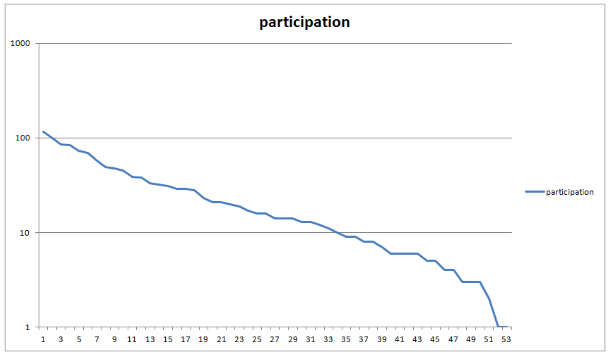
\includegraphics[scale=0.75]{img/Visual_represntation_1.PNG}} %[width=0.7\textwidth]
\caption{Visual representation of user participation in EvoDrawing01.}
\label{fig:userP_1}
\end{figure*}

Figure \ref{fig:userP_1}  a visual representation of user
participation is presented, this experiment where the y-axis represents the level of
participation and the x-axis represents the number of users who participated in
this experiment.

\begin{figure*}
%\captionsetup{justification=centering,margin=1cm}
\centering
\fbox{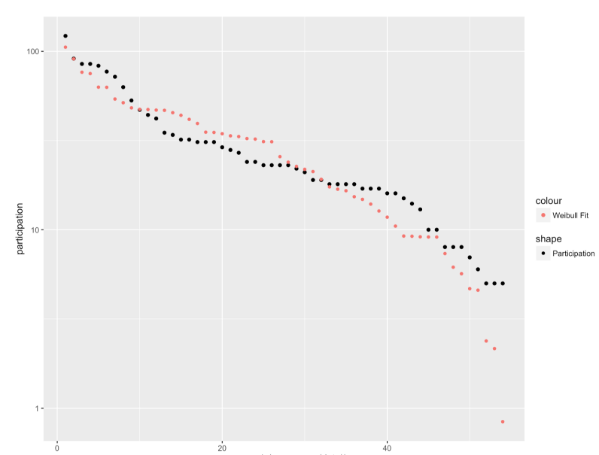
\includegraphics[scale=0.75]{img/weibull_1.PNG}} %[width=0.7\textwidth]
\caption{Weibull fit data representation.}
\label{fig:weibull_1}
\end{figure*}

For this particular experiment we were modeling with the Weibull distribution
\cite{weibull1951wide} the participation data of 53 users and these are the
results of the shape parameter and those of scale:

\begin{table}
\small
\caption{Weibull parameters.}
\label{tab:weibullp_1}
\centering
\small
\begin{tabular}{p{3cm} p{3cm} p{3cm} }
\hline\noalign{\smallskip}
Shape  & Scale &  \\
\noalign{\smallskip}\hline\noalign{\smallskip}
\small{0.9940324} & \small{25.4201542} & \\ \hline
\small{( 0.1036683)} & \small{( 3.7182494)} & \\ \hline

\noalign{\smallskip}\hline
\end{tabular}
\end{table}

Table \ref{tab:weibullp_1} shows the behavior in the Figure
\ref{fig:userP_1}, where the red dots are the adjustment of the Weibull
distribution and the black dots are the real data of the participations of the
users.



\section {EvoDrawing02}



Table \ref{tab:dataGenerated_2} shows the nodes and relatioships generated
by experiment ED02.

\begin{table}
\small
\caption{Data generated in graph-based user modeling.}
\label{tab:dataGenerated_2}
\centering
\small
\begin{tabular}{p{3cm} p{3cm} p{3cm} }
\hline\noalign{\smallskip}
  & Data &  \\
\noalign{\smallskip}\hline\noalign{\smallskip}
\small{Nodes} & \small{648} & \\ \hline
\small{Relationships} & \small{2596} & \\ \hline

\noalign{\smallskip}\hline
\end{tabular}
\end{table}
Also, the table\ref{tab:totalUsers_1} is the total of volunteer active users is
presented.

The total number of users who participate voluntarily is shown in the table \ref{tab:totalUsers_1}.

\begin{table}
\small
\caption{Total number of volunteers active users.}
\label{tab:totalUsers_1}
\centering
\small
\begin{tabular}{p{3cm} p{3cm} p{3cm} }
\hline\noalign{\smallskip}
  & Users &  \\
\noalign{\smallskip}\hline\noalign{\smallskip}
\small{Total } & \small{54} & \\ \hline
\noalign{\smallskip}\hline
\end{tabular}
\end{table}

Like in the previous experiment, in which we wanted to observe which users
had better social
interconnectivity within the experiment, it was decided to see this
relationship that corresponds to the number of known users. The table \ref{tab:totalUsers_1}
showed the relationships where the top 10 user  with social
interconnectivity for this particular experiment.


\begin{table}
\small
\caption{A sample of the top 10 users interconnected users.}
\label{tab:knownUsers_2}
\centering
\small
\begin{tabular}{p{3cm} p{3cm}  }
\hline\noalign{\smallskip}
 User name & Number of known users \\
\noalign{\smallskip}\hline\noalign{\smallskip}
\small{Rogelio UR} & \small{10}  \\ \hline
\small{Barbara Sandoval} & \small{9}  \\ \hline
\small{Evelyn Macedo} & \small{8}  \\ \hline
\small{Chriss de Blanc} & \small{8}  \\ \hline
\small{Cesar Rojas} & \small{8}  \\ \hline
\small{Jasiel Calzada} & \small{8}  \\ \hline
\small{Tonyy Maldonado} & \small{7}  \\ \hline
\small{Silvano Peraza} & \small{7}  \\ \hline
\small{Hector Beltran Medrano} & \small{6}  \\ \hline
\small{Juan Ferman Lopez} & \small{6}  \\ \hline
\noalign{\smallskip}\hline
\end{tabular}
\end{table}

Figure \ref{fig:userInter_2} shows users with more interconnectivity in the
graph. This may represent a certain degree of impact of a user and a possible influence
that may have on the decisions of other users. For example, if the
user with the greatest impact is affected in any decision likely other users may
be affected in some way. Particularly in this experiment the degree of social
interconnectivity among users is becoming more complex as compared to the
previous experiment.

\begin{figure*}
%\captionsetup{justification=centering,margin=1cm}
\centering
\fbox{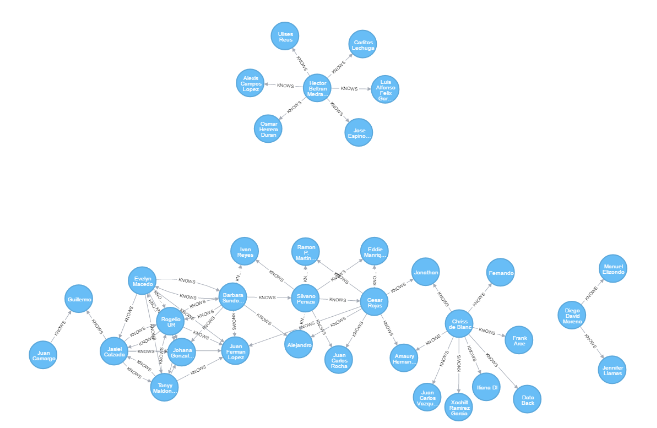
\includegraphics[scale=0.75]{img/user_known_2.PNG}} %[width=0.7\textwidth]
\caption{Graph users with greater interconnectivity.}
\label{fig:userInter_2}
\end{figure*}

\begin{table}
\small
\caption{Sample of 30 individuals evaluated from.}
\label{tab:totalIndividuals_2}
\centering
\small
\begin{tabular}{p{3cm} p{4cm} p{3cm} p{3cm}}
\hline\noalign{\smallskip}
 id & Chromosome & Views & Likes  \\
\noalign{\smallskip}\hline\noalign{\smallskip}
\small{pop:individual:55} & \small{[63, 58, 0, 1, 1, 1, 4, 0, 0, 1, 0, 0, 0, 0, 3]}
& \small{18} & \small{18}\\ \hline
\small{pop:individual:329} & \small{[98, 37, 0, 1, 1, 0, 4, 0, 0, 1, 0, 0, 0, 0, 2]}
& \small{17} & \small{17}\\ \hline
\small{pop:individual:304} & \small{[63, 58, 0, 1, 1, 1, 4, 0, 0, 0, 3, 0, 0, 2, 2]}
& \small{16} & \small{16}\\ \hline
\small{pop:individual:202} & \small{[107, 79, 1, 0, 1, 1, 3, 0, 0, 1, 3, 0, 1, 1]}
& \small{15} & \small{15}\\ \hline
\small{pop:individual:58} & \small{[150, 79, 1, 0, 1, 1, 3, 0, 0, 1, 3, 0, 1, 1, 1]}
& \small{14} & \small{14}\\ \hline
\small{pop:individual:310} & \small{[63, 58, 0, 1, 1, 1, 4, 0, 0, 1, 0, 0, 1, 2, 2]}
& \small{13} & \small{13}\\ \hline
\small{pop:individual:67} & \small{[65, 51, 1, 1, 0, 0, 3, 1, 0, 0, 3, 1, 0, 2, 3]}
& \small{12} & \small{12}\\ \hline
\small{pop:individual:48} & \small{[51, 73, 0, 0, 0, 0, 2, 0, 0, 1, 3, 0, 1, 0, 3]}
& \small{12} & \small{12}\\ \hline
\small{pop:individual:179} & \small{[98, 37, 0, 1, 1, 1, 4, 0, 0, 1, 0, 0, 0, 0, 3]}
& \small{12} & \small{12}\\ \hline
\small{pop:individual:114} & \small{[63, 58, 0, 1, 1, 1, 4, 0, 0, 1, 0, 0, 0, 0, 2]}
& \small{12} & \small{12}\\ \hline
\small{pop:individual:123} & \small{[124, 42, 0, 1, 1, 1, 4, 1, 0, 1, 1, 0, 0, 2, 1]}
& \small{12} & \small{12}\\ \hline
\small{pop:individual:344} & \small{[97, 66, 0, 0, 1, 1, 3, 0, 1, 0, 3, 0, 1, 0, 1]}
& \small{11} & \small{11}\\ \hline
\small{pop:individual:105} & \small{[63, 58, 0, 1, 1, 1, 4, 0, 0, 1, 0, 0, 0, 0, 2]}
& \small{11} & \small{11}\\ \hline
\small{pop:individual:435} & \small{[98, 37, 0, 1, 1, 0, 1, 1, 4, 1, 0, 0, 0, 0, 2]}
& \small{11} & \small{11}\\ \hline
\small{pop:individual:140} & \small{[150, 79, 1, 0, 1, 1, 3, 1, 1, 0, 1, 1, 1, 2, 3]}
& \small{11} & \small{11}\\ \hline
\small{pop:individual:216} & \small{[124, 42, 0, 1, 0, 0, 3, 0, 0, 1, 1, 0, 0, 1, 1]}
& \small{11} & \small{11}\\ \hline
\small{pop:individual:290} & \small{[150, 79, 1, 0, 1, 1, 3, 0, 0, 1, 3, 0, 1, 0, 1]}
& \small{10} & \small{10}\\ \hline
\small{pop:individual:255} & \small{[150, 79, 1, 0, 1, 1, 3, 1, 1, 1, 0, 0, 1, 2, 2]}
& \small{10} & \small{10}\\ \hline
\small{pop:individual:14} & \small{[89, 66, 0, 0, 1, 1, 3, 0, 0, 0, 2, 0, 0, 2, 1]}
& \small{10} & \small{10}\\ \hline
\small{pop:individual:366} & \small{[128, 66, 0, 1, 1, 4, 1, 0, 1, 0, 0, 0, 1, 2, 2]}
& \small{10} & \small{10}\\ \hline
\small{pop:individual:215} & \small{[54, 72, 0, 1, 1, 1, 4, 0, 0, 1, 0, 0, 0, 0, 2]}
& \small{9} & \small{9}\\ \hline
\small{pop:individual:411} & \small{[113, 58, 0, 1, 1, 1, 4, 0, 0, 1, 0, 0, 1, 2, 2]}
& \small{9} & \small{9}\\ \hline
\small{pop:individual:254} & \small{[113, 58, 0, 1, 1, 4, 1, 0, 4, 1, 1, 0, 0, 3]}
& \small{11} & \small{9}\\ \hline
\small{pop:individual:285} & \small{[54, 58, 0, 0, 0, 1, 1, 4, 1, 1, 0, 0, 1, 2, 2]}
& \small{8} & \small{8}\\ \hline
\small{pop:individual:500} & \small{[63, 58, 1, 1, 1, 0, 3, 0, 1, 1, 0, 0, 1, 2, 0]}
& \small{8} & \small{8}\\ \hline
\small{pop:individual:415} & \small{[54, 72, 0, 1, 1, 1, 4, 1, 4, 1, 3, 0, 1, 1]}
& \small{8} & \small{8}\\ \hline
\small{pop:individual:300} & \small{[54, 58, 1, 0, 1, 1, 1, 4, 1, 1, 0, 0, 1, 2, 2]}
& \small{8} & \small{8}\\ \hline
\small{pop:individual:32} & \small{[113, 29, 0, 0, 0, 0, 4, 1, 0, 1, 0, 1, 1, 1, 3]}
& \small{8} & \small{8}\\ \hline
\small{pop:individual:237} & \small{[63, 58, 1, 1, 0, 1, 1, 4, 1, 0, 0, 0, 1, 2, 3]}
& \small{8} & \small{8}\\ \hline
\small{pop:individual:268} & \small{[98, 37, 0, 1, 1, 1, 4, 0, 0, 1, 0, 0, 0, 0]}
& \small{8} & \small{8}\\ \hline
\noalign{\smallskip}\hline
\end{tabular}
\end{table}

Table \ref{tab:totalIndividuals_2} contains a sample of individuals 30/556
generated in the experiment. This table shows the unique identifier of the
individual, its chromosome, as well as the number of views, likes available to
the individual. These results are useful to observe individuals have been better
evaluated by users.

\begin{table}
\small
\caption{Level of user participation.}
\label{tab:userParticipation_2}
\centering
\small
\begin{tabular}{p{4cm} p{4cm}}
\hline\noalign{\smallskip}
 User name & Participation   \\
\noalign{\smallskip}\hline\noalign{\smallskip}
\small{1122212314475816} & \small{122} \\ \hline
\small{1107674982600275} & \small{91} \\ \hline
\small{10207544086753085} & \small{86} \\ \hline
\small{1128990193799346} & \small{85} \\ \hline
\small{1067084180030552} & \small{83} \\ \hline
\small{985591718197586} & \small{77} \\ \hline
\small{969507913124553} & \small{72} \\ \hline
\small{10207004677610003} & \small{63} \\ \hline
\small{1223229694371825} & \small{53} \\ \hline
\small{10153904046011462} & \small{47} \\ \hline
\small{1032494570125948} & \small{44} \\ \hline
\small{995610090523549} & \small{42} \\ \hline
\small{975038365907627} & \small{35} \\ \hline
\small{10207487295119454} & \small{34} \\ \hline
\small{1041989022528624} & \small{32} \\ \hline
\small{471974623003503} & \small{32} \\ \hline
\small{1275844349097672} & \small{31} \\ \hline
\small{978744228875903} & \small{31} \\ \hline
\small{10205734318020434} & \small{31} \\ \hline
\small{10209454397419860} & \small{29} \\ \hline


\noalign{\smallskip}\hline
\end{tabular}
\end{table}

Table \ref{tab:userParticipation_2} shows the results of the level of user
participation in the experiment. These were obtained by counting the vicinity of
nearest nodes from the base node, in this case, each user node.


\begin{figure*}
%\captionsetup{justification=centering,margin=1cm}
\centering
\fbox{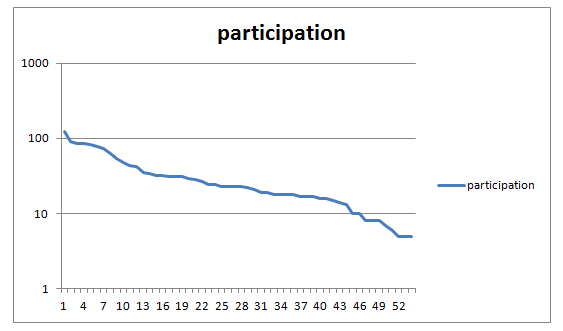
\includegraphics[scale=0.75]{img/visual_representation_2.PNG}} %[width=0.7\textwidth]
\caption{Visual representation of user participation in EvoDrawing01.}
\label{fig:userP_2}
\end{figure*}


Figure \ref{fig:userP_2} shows a visual representation of user
participation in this experiment where the y-axis represents the level of
participation and the x-axis represents the number of users who participated in
this experiment.

\begin{figure*}
%\captionsetup{justification=centering,margin=1cm}
\centering
\fbox{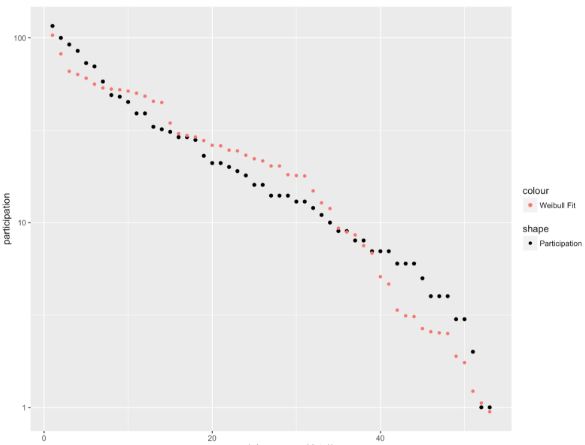
\includegraphics[scale=0.75]{img/weibull_2.PNG}} %[width=0.7\textwidth]
\caption{Weibull fit data representation.}
\label{fig:weibull_2}
\end{figure*}

For this particular experiment we were modeling with the Weibull distribution
\cite{weibull1951wide} the participation data of 54 users and these are the
results of the shape and the scale parameter:

\begin{table}
\small
\caption{Weibull parameters.}
\label{tab:weibullp_2}
\centering
\small
\begin{tabular}{p{3cm} p{3cm} p{3cm} }
\hline\noalign{\smallskip}
Shape  & Scale &  \\
\noalign{\smallskip}\hline\noalign{\smallskip}
\small{1.3255300} & \small{33.7680210} & \\ \hline
\small{(0.1330041)} & \small{(3.6776628)} & \\ \hline

\noalign{\smallskip}\hline
\end{tabular}
\end{table}

Table \ref{tab:weibullp_2} shows the behavior, Figure
\ref{fig:weibull_2} show Weibull distribution, where the red dots are the adjustment of the Weibull
distribution and the black dots are the real data of the participations of the
users.




\section{EvoDrawing03}
In the experiment ED03 the following data were
generated presented in \ref{tab:dataGenerated_3}.

\begin{table}
\small
\caption{Data generated in graph-based user modeling.}
\label{tab:dataGenerated_3}
\centering
\small
\begin{tabular}{p{3cm} p{3cm} p{3cm} }
\hline\noalign{\smallskip}
  & Data &  \\
\noalign{\smallskip}\hline\noalign{\smallskip}
\small{Nodes} & \small{3746 } & \\ \hline
\small{Relationships} & \small{17207 } & \\ \hline

\noalign{\smallskip}\hline
\end{tabular}
\end{table}

The total number of users who participate voluntarily shown in \ref{tab:totalUsers_3}.

\begin{table}
\small
\caption{Total number of volunteers active users.}
\label{tab:totalUsers_3}
\centering
\small
\begin{tabular}{p{3cm} p{3cm} p{3cm} }
\hline\noalign{\smallskip}
  & Users &  \\
\noalign{\smallskip}\hline\noalign{\smallskip}
\small{Total } & \small{68} & \\ \hline
\noalign{\smallskip}\hline
\end{tabular}
\end{table}

In the same way as the previous experiment, which wanted to observe users, had
better social interconnectivity within this experiment, it was decided a known
ratio of the number of users that have. This relationship is presented in Table
\ref{tab:knownUsers_3}  where we show the 10 users with better social
interconnectivity.

\begin{table}
\small
\caption{A sample of the top 10 users level influence on users.}
\label{tab:knownUsers_3}
\centering
\small
\begin{tabular}{p{3cm} p{3cm}  }
\hline\noalign{\smallskip}
 User name & Number of known users \\
\noalign{\smallskip}\hline\noalign{\smallskip}
\small{David Astorga Viramontes} & \small{23}  \\ \hline
\small{Evelyn Macedo} & \small{18}  \\ \hline
\small{Reyes Zuniga} & \small{17}  \\ \hline
\small{Barbara Sandoval} & \small{16}  \\ \hline
\small{Chriss de Blanc} & \small{15}  \\ \hline
\small{Luis Alfonso Felix Garcia} & \small{15}  \\ \hline
\small{Paulina NG} & \small{15}  \\ \hline
\small{Marco Antonio Fuentes Alvarez} & \small{15}  \\ \hline
\small{Jasiel Calzada} & \small{14}  \\ \hline
\small{Hector Beltran Medrano} & \small{13}  \\ \hline
\noalign{\smallskip}\hline
\end{tabular}
\end{table}


\begin{figure*}
%\captionsetup{justification=centering,margin=1cm}
\centering
\fbox{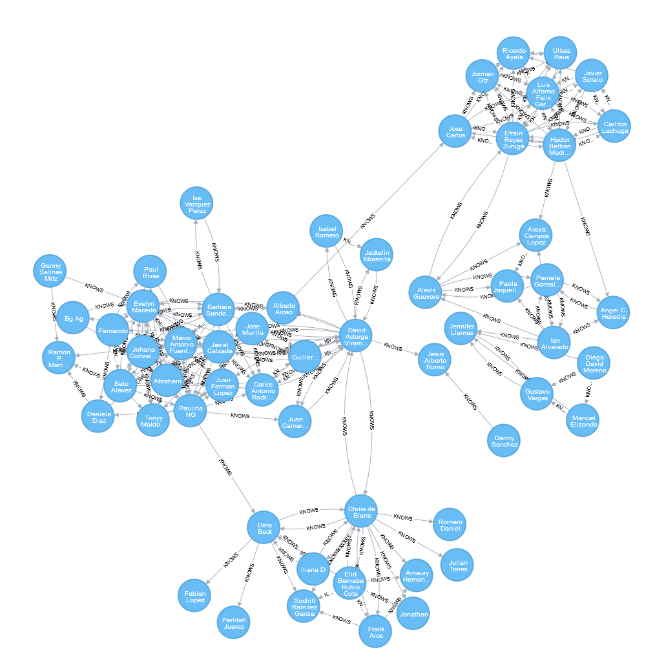
\includegraphics[scale=0.75]{img/user_known_3.PNG}} %[width=0.7\textwidth]
\caption{Social interconnectivity in graph-based user model.}
\label{fig:graphKnown_3}
\end{figure*}

Figure \ref{fig:graphKnown_3} shows users more connected in the graph. This
may represent a degree of impact of a user and the possible influence that may
have on the decisions of other users. For example, if the user with the greatest
impact is affected in any decision likely other users may be affected in some
way. Particularly in this experiment the social graph interconnectivity among
users is becoming more complex as compared to the previous experiment as we can
observe that more closely resembles a social network.


\begin{table}
\small
\caption{Total number of individuals.}
\label{tab:totalIndividuals_33}
\centering
\small
\begin{tabular}{p{3cm} p{3cm} p{3cm} }
\hline\noalign{\smallskip}
  & Individuals &  \\
\noalign{\smallskip}\hline\noalign{\smallskip}
\small{Total } & \small{3594} & \\ \hline
\noalign{\smallskip}\hline
\end{tabular}
\end{table}

Table \ref{tab:totalIndividuals_33} shows the total number of individuals
evaluated by users in this experiment.

\begin{table}
\small
\caption{Sample of 30 individuals evaluated from.}
\label{tab:totalIndividuals_32}
\centering
\small
\begin{tabular}{p{3cm} p{4cm} p{3cm} p{3cm}}
\hline\noalign{\smallskip}
 id & Chromosome & Views & Likes  \\
\noalign{\smallskip}\hline\noalign{\smallskip}
\small{pop:individual:3570} & \small{[113, 44, 0, 1, 0, 0, 1, 0, 1, 0, 3, 1, 1, 0, 1]}
& \small{48} & \small{48}\\ \hline
\small{pop:individual:3544} & \small{[150, 44, 0, 0, 1, 1, 1, 0, 0, 1, 1, 0, 1, 0, 0]}
& \small{32} & \small{26}\\ \hline
\small{pop:individual:210} & \small{[63, 58, 0, 1, 1, 1, 4, 0, 0, 0, 3, 0, 0, 2, 2]}
& \small{16} & \small{16}\\ \hline
\small{pop:individual:202} & \small{[113, 5, 0, 1, 1, 0, 4, 0, 1, 1, 2, 1, 0, 2, 2]}
& \small{22} & \small{22}\\ \hline
\small{pop:individual:58} & \small{[61, 70, 0, 0, 1, 0, 1, 0, 0, 0, 2, 0, 1, 0, 3]}
& \small{23} & \small{21}\\ \hline
\small{pop:individual:858} & \small{[113, 1, 1, 1, 1, 0, 1, 1, 1, 3, 0, 1, 1, 0]}
& \small{21} & \small{21}\\ \hline
\small{pop:individual:17} & \small{[113, 69, 0, 1, 1, 1, 3, 0, 1, 1, 0, 0, 1, 0, 3]}
& \small{23} & \small{21}\\ \hline
\small{pop:individual:3636} & \small{[118, 44, 0, 0, 1, 1, 1, 0, 0, 1, 1, 1, 1, 0, 0]}
& \small{22} & \small{21}\\ \hline
\small{pop:individual:33} & \small{[129, 79, 0, 1, 1, 0, 1, 1, 0, 0, 0, 1, 0, 0, 1]}
& \small{20} & \small{20}\\ \hline
\small{pop:individual:74} & \small{[150, 50, 1, 1, 1, 1, 1, 1, 0, 1, 3, 1, 0, 1, 3]}
& \small{21} & \small{19}\\ \hline
\small{pop:individual:65} & \small{[94, 62, 1, 0, 0, 0, 2, 0, 1, 0, 3, 0, 1, 2, 2]}
& \small{20} & \small{19}\\ \hline
\small{pop:individual:50} & \small{[50, 70, 0, 1, 1, 1, 3, 1, 1, 1, 1, 1, 1, 1, 3]}
& \small{19} & \small{19}\\ \hline
\small{pop:individual:52} & \small{[131, 63, 1, 1, 1, 0, 4, 0, 1, 1, 0, 0, 1, 0, 3]}
& \small{20} & \small{19}\\ \hline
\small{pop:individual:2449} & \small{[113, 44, 0, 1, 1, 1, 1, 0, 1, 1, 0, 0, 1, 1, 2]}
& \small{18} & \small{18}\\ \hline
\small{pop:individual:44} & \small{[117, 54, 0, 0, 0, 0, 2, 0, 1, 1, 3, 1, 0, 2, 3]}
& \small{19} & \small{18}\\ \hline
\small{pop:individual:113} & \small{[77, 21, 1, 0, 1, 0, 4, 0, 1, 0, 0, 1, 0, 3]}
& \small{17} & \small{17}\\ \hline
\small{pop:individual:84} & \small{[102, 69, 1, 0, 1, 0, 3, 0, 0, 0, 0, 0, 1, 0, 3]}
& \small{17} & \small{17}\\ \hline
\small{pop:individual:95} & \small{[68, 43, 0, 1, 0, 1, 3, 1, 0, 0, 3, 0, 0, 1, 2]}
& \small{19} & \small{16}\\ \hline
\small{pop:individual:22} & \small{[137, 20, 0, 0, 0, 0, 0, 1, 0, 0, 3, 0, 1, 1, 1]}
& \small{17} & \small{16}\\ \hline
\small{pop:individual:71} & \small{[79, 5, 0, 0, 1, 1, 2, 1, 0, 1, 0, 1, 1, 1, 3]}
& \small{16} & \small{16}\\ \hline
\small{pop:individual:42} & \small{[112, 35, 1, 0, 1, 0, 1, 0, 1, 0, 0, 1, 1, 0, 2]}
& \small{9} & \small{9}\\ \hline
\small{pop:individual:411} & \small{[113, 58, 0, 1, 1, 1, 4, 0, 0, 1, 0, 0, 1, 2, 2]}
& \small{16} & \small{15}\\ \hline
\small{pop:individual:59} & \small{[93, 23, 0, 0, 0, 1, 4, 0, 0, 0, 1, 0, 1, 2, 1]}
& \small{17} & \small{15}\\ \hline
\small{pop:individual:40} & \small{[137, 9, 1, 0, 1, 0, 3, 0, 1, 1, 2, 0, 1, 2, 1]}
& \small{15} & \small{15}\\ \hline
\small{pop:individual:85} & \small{[120, 42, 0, 1, 0, 1, 0, 0, 1, 1, 3, 0, 1, 1, 2]}
& \small{16} & \small{15}\\ \hline
\small{pop:individual:90} & \small{[130, 76, 0, 0, 1, 1, 1, 1, 1, 1, 1, 0, 1, 2, 3]}
& \small{15} & \small{15}\\ \hline
\small{pop:individual:73} & \small{[88, 67, 0, 0, 0, 0, 0, 1, 1, 1, 2, 1, 0, 1, 3]}
& \small{15} & \small{15}\\ \hline
\small{pop:individual:943} & \small{[116, 44, 0, 0, 0, 4, 1, 1, 1, 1, 0, 1, 0, 1, 1]}
& \small{15} & \small{15}\\ \hline
\small{pop:individual:353} & \small{[121, 20, 1, 1, 0, 0, 1, 0, 1, 1, 3, 0, 1, 0, 2]}
& \small{15} & \small{15}\\ \hline
\small{pop:individual:79} & \small{[68, 5, 1, 1, 0, 1, 1, 1, 1, 0, 2, 1, 1, 1, 1]}
& \small{14} & \small{14}\\ \hline
\noalign{\smallskip}\hline
\end{tabular}
\end{table}

Table \ref{tab:totalIndividuals_32} contains a sample of individuals 30/556
generated in the experiment. In this, its a unique identifier of the individual,
its chromosome, as well as the number of views, likes available to the individual presents.
This results, which are useful to observe individuals have been better evaluated by users.

\begin{table}
\small
\caption{Level of user participation.}
\label{tab:userParticipation_22}
\centering
\small
\begin{tabular}{p{4cm} p{4cm}}
\hline\noalign{\smallskip}
 User name & Participation   \\
\noalign{\smallskip}\hline\noalign{\smallskip}
\small{1157401414272355} & \small{2035} \\ \hline
\small{1001585659925992} & \small{1828} \\ \hline
\small{1244770712203948} & \small{1722} \\ \hline
\small{990632971026794} & \small{552} \\ \hline
\small{987920194610578} & \small{456} \\ \hline
\small{10207675081608741} & \small{300} \\ \hline
\small{966757780068615} & \small{267} \\ \hline
\small{1228561717171956} & \small{258} \\ \hline
\small{985416538190778} & \small{203} \\ \hline
\small{1123938694291507} & \small{202} \\ \hline
\small{10207552420841432} & \small{200} \\ \hline
\small{1124138344283213} & \small{169} \\ \hline
\small{220415891643957} & \small{161} \\ \hline
\small{534039336778842} & \small{112} \\ \hline
\small{10153940958696462} & \small{93} \\ \hline
\small{10205543461172072} & \small{87} \\ \hline
\small{1281817738500333} & \small{81} \\ \hline
\small{10153866481615259} & \small{74} \\ \hline
\small{943775989063530} & \small{73} \\ \hline
\small{10205664691039169} & \small{71} \\ \hline


\noalign{\smallskip}\hline
\end{tabular}
\end{table}

Figure \ref{fig:userP_3} shows a visual representation of user participation
of this experiment where the y-axis represents the level of participation and
the x-axis represents the number of users who participated in this experiment.

\begin{figure*}
%\captionsetup{justification=centering,margin=1cm}
\centering
\fbox{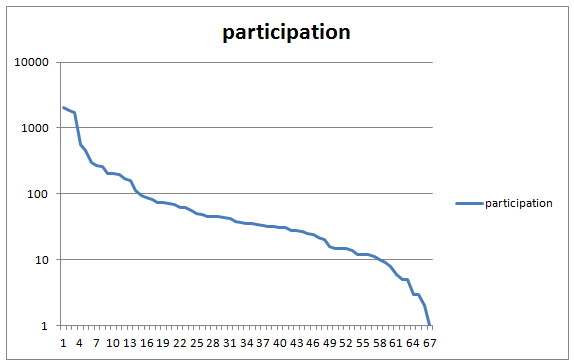
\includegraphics[scale=0.75]{img/visual_representation_3.PNG}} %[width=0.7\textwidth]
\caption{Visual representation of user participation in EvoDrawing01.}
\label{fig:userP_3}
\end{figure*}


\begin{figure*}
%\captionsetup{justification=centering,margin=1cm}
\centering
\fbox{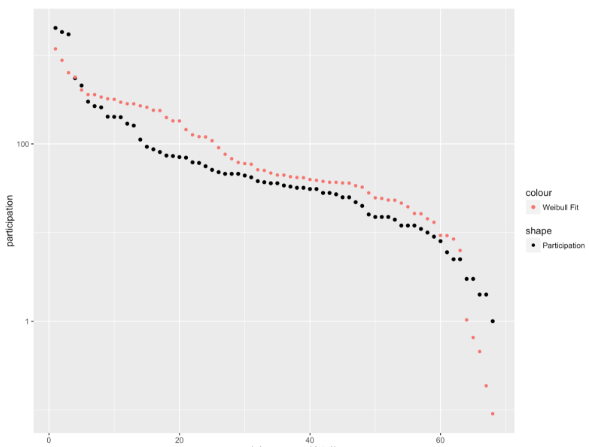
\includegraphics[scale=0.75]{img/weibull_3.PNG}} %[width=0.7\textwidth]
\caption{Weibull fit data representation.}
\label{fig:weibull_3}
\end{figure*}

For this particular experiment we were modeling with the Weibull distribution
\cite{weibull1951wide} the participation data of 68 users and these are the
results of the shape and scale parameter:

\begin{table}
\small
\caption{Weibull parameters.}
\label{tab:weibullp_3}
\centering
\small
\begin{tabular}{p{3cm} p{3cm} p{3cm} }
\hline\noalign{\smallskip}
Shape  & Scale &  \\
\noalign{\smallskip}\hline\noalign{\smallskip}
\small{0.6027560} & \small{85.0232792} & \\ \hline
\small{(0.0507141)} & \small{(18.1151136)} & \\ \hline

\noalign{\smallskip}\hline
\end{tabular}
\end{table}

Table \ref{tab:weibullp_3} shows the behavior in the Figure
\ref{fig:weibull_3}, where the red dots are the adjustment of the Weibull
distribution and the black dots are the real data of the participations of the
users.



\section{Comparison between experiments.}
Figure \ref{fig:comparison} shows a comparative chart of the results obtained
in the three phases of the study case, each of the lines on the graph represents
one of the versions of EvoDrawing in relation to the number of units of users
that were obtained are presented in different experiments. For instance the blue
line represents ED1 experiment, the red line represents ED02
and finally the green line represents ED03.


\begin{figure*}
%\captionsetup{justification=centering,margin=1cm}
\centering
\fbox{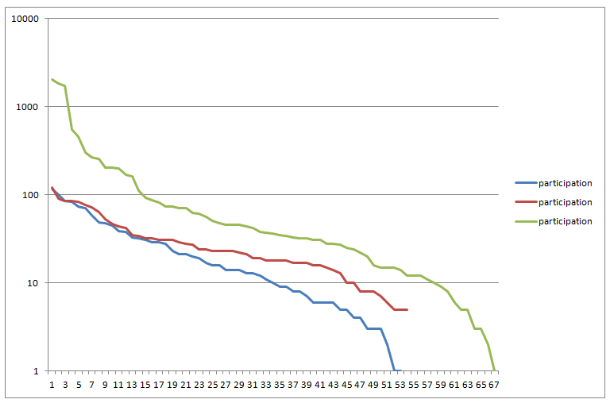
\includegraphics[scale=0.75]{img/comparison.PNG}} %[width=0.7\textwidth]
\caption{Graphical representation of user participation in the different experiments.}
\label{fig:comparison}
\end{figure*}
